\section{Анализ предметной области}

В данной главе будет дан обзор системы типов языка Kotlin, описаны некоторый её проблемы и возможные решения.
После будет введено понятие Self-типа и показаны его преимущества как потенциального решения обозначенных проблем.
В завершение будут приведены приложения Self-типов как возможности типовой системы языка Kotlin.

\subsection{Система типов языка Kotlin}

\begin{definition}
    \term{Kotlin} --- это компилируемый промышленный язык программирования, поддерживающий компиляцию в Java bytecode, JavaScript и нативный код\cite{jemerov2017kotlin}.
\end{definition}

\begin{definition}
    \term{Система типов} --- это гибко управляемый синтаксический метод доказательства отсутствия в программе определенных видов поведения при помощи классификации выражений языка по разновидностям вычисляемых ими значений\cite{pierce2002types}.
\end{definition}

Система типов языка программирования Kotlin обладает следующими основными свойствами\cite{akhin2021kotlin}.
\begin{itemize}
    \item Статическая --- проверка типов происходит на этапе компиляции;
    \item Gradual --- система типов может накладывать более слабые ограничения, делегируя проверку типов времени исполнения программы, для лучшей поддержки взаимодействия с кодом целевой платформы (реализуется в Kotlin с помощью \term{flixible types})\cite{siek2007gradual};
    \item Flow --- типизация значений в программе может зависеть от графа потока управления (реализуется в Kotlin через механизм \term{smart-casts})\cite{pearce2013calculus}\ref{subsubsec:smart-casts};
    \item Null-безопасная --- вводится две вселенные типов: типы, которые содержат значение \mintinline{kotlin}|null|, и которые \mintinline{kotlin}|null| не содержат;
    \item Без небезопасных неявных типовых конверсий;
    \item С общими верхним и нижним типами относительно отношения подтипизации --- тип \mintinline{kotlin}|Nothing| является подтипом любого типа, а \mintinline{kotlin}|Any?| --- супертипом любого типа;
    \item С номинальной подтипизацией --- один тип является подтипом другого только в случае явного указания программиста;
    \item С ограниченным параметрическим полиморфизмом и поддержкой вариантности\ref{subsubsec:variance}.
\end{itemize}

\subsubsection{Наследование и виртуальный полиморфизм}

\begin{definition}
    \label{def:subtype}
    Тип \texttt{B} является \term{подтипом} типа \texttt{A} тогда и только тогда, когда значение типа \texttt{B} можно присвоить в переменную типа \texttt{A}.
    Тип \texttt{A} называют \term{супертипом} (или \term{базовым типом}) типа \texttt{B}.
    Обозначение \texttt{B <: A}.
\end{definition}

Система типов языка Kotlin является \term{номинативной}.
Это значит, что отношение подтипизации нужно указывать явно и оно не следует из структуры значений типа.
Основным способом задания отношения подтипизации в Kotlin является \term{наследование}.

С помощью наследования же в Kotlin реализуется \term{виртуальный полиморфизм}.
Он заключается в том, что по ссылке базового типа происходит вызов метода наследника, если в действительность это ссылка на метод наследника.
\begin{minted}{kotlin}
    open class Base {
        fun method() { println("Base") }
    }

    class Derived : Base() {
        override fun method() { println("Derived") }
    }

    fun test() {
        val base: Base = Derived()
        base.method() // Печатает "Derived"
    }
\end{minted}

\subsubsection{Smart-casts}\label{subsubsec:smart-casts}

\begin{definition}
    \label{def:basic-block}
    \term{Базовый блок} --- непрерывная последовательность инструкций, всегда выполняющихся последовательно.
\end{definition}

\begin{definition}
    \label{def:cfg}
    \term{Граф потока управления программы (CFG --- control flow graph)} --- граф, составленный по программе из её базовых блоков.
    На рисунке~\ref{fig:cfg-example} приведён пример графа потока управления.
\end{definition}

\begin{figure}
    \centering
    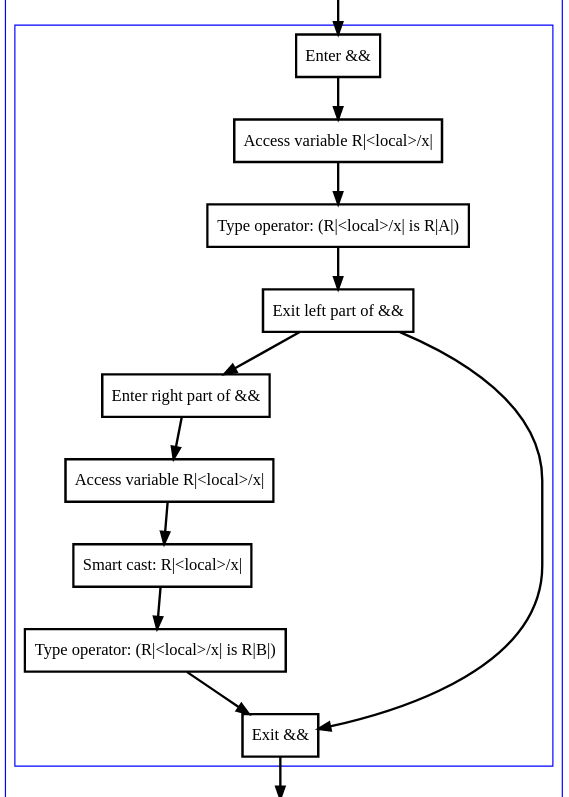
\includegraphics[width=0.8\linewidth]{fig/cfgExample}
    %! suppress = EscapeAmpersand
    \caption{Граф потока управления выражения \mintinline{kotlin}|x is A && x is B|.}
    \label{fig:cfg-example}
\end{figure}

\begin{definition}
    \label{def:intersection-types}
    \term{Тип-пересечение} --- тип, являющийся подтипом одновременно всех типов из пересечения.
    Обозначение для пересечения типов \texttt{A}, \texttt{B} и \texttt{C}: \texttt{A \& B \& C}.
\end{definition}

Типы-пересечения являются примером типов, которые нельзя записать в Kotlin, то есть они не доступны программисту, но возникают в процессе вывода типов.
\begin{minted}{kotlin}
    interface A {
        fun aMethod() { /* ... */ }
    }

    interface B {
        fun bMethod() { /* ... */ }
    }

    class C : A, B
    class D : A, B

    fun test(cond: Boolean) {
        val intersection /* : A & B */ = if (b) C() else D()
        intersection.aMethod() // ok
        intersection.bMethod() // ok
    }
\end{minted}

\begin{definition}
    \term{Smart-casts} --- механизм уточнения типа за счёт информации, получаемой из графа потока управления программы.
\end{definition}

Например, если в условной конструкции проверяется принадлежность значения переменной типу, то в теле доступна информация о том, что тип этой переменной включает в себя тип из условия.
Это выражается с помощью типов-пересечений~\ref{def:intersection-types}.

\begin{minted}{kotlin}
    fun test(x: A) {
        if (x is B) {
            // x: A & B
            #\colorbox{green}{x}#.bMethod()
        }
    }
\end{minted}

\subsubsection{Параметрический полиморфизм и вариантность}\label{subsubsec:variance}

\begin{definition}
    \label{def:param-poly}
    \term{Параметрический полиморфизм} --- способность функции или класса работать с объектами различных типов путём абстрагирования реализации по типовому параметру.
\end{definition}

\begin{definition}
    \term{Ограниченный параметрический полиморфизм}~--- параметрический полиморфизм, поддерживающий добавление ограничений на типы, которые можно использовать как типовые аргументы.
    В случае Kotlin, данным ограничением является наличие определённого супертипа.
\end{definition}

\begin{definition}
    \term{Вариантность} --- механизм языков с параметрическим полиморфизмом, позволяющий дополнять отношение подтипизации между параметризованными типами, когда аргументы --- разные типы, связанные в свою очередь отношением подтипизации.
\end{definition}

В Kotlin вариантность может сообщаться как типовому параметру класса, так и в месте использования этого класса.
В нашем изложении мы ограничимся только первым случаем, второй рассматривается аналогично.

\begin{definition}\label{def:invariant}
    \term{Инвариантный типовой параметр} --- может использоваться в произвольных позициях деклараций методов класса.
    Не дополняет отношение подтипизации между параметризованными типами.
\end{definition}

Так, если имеется определение \mintinline[escapeinside=??]{kotlin}|interface Inv<T> { fun id(x: ?\framebox{T}?): ?\framebox{T}? }|, отношение подтипизации не образуется ни для каких \texttt{A} и \texttt{B}: \mintinline{kotlin}|Inv<A> !<:> Inv<B>|.

\begin{definition}\label{def:covariant}
    \term{Ковариантный типовой параметр} --- может использоваться как исходящих позициях деклараций методов класса, так и как типовой аргумент других типовых параметров в ковариантных позициях.
    Параметризованный тип образует такое же отношение подтипизации, что и типовые параметры.
\end{definition}

Пусть \mintinline[escapeinside=??]{kotlin}|interface Out<?\framebox{out}? T> { fun produce(): ?\framebox{T}? }|, тогда если \texttt{B <: A}, то \texttt{Out<B> <: Out<A>}.

TODO % TODO

\subsubsection{Ресиверы}

TODO % TODO

\subsubsection{Типовые скоупы}

TODO % TODO
